\section{M. Diehl, Wieber - Fast direct multiple shooting algorithms for optimal robot control \cite{DiehlWieber}}
year: 2009

Optimal control problems can be devided in the following way:
\begin{itemize}
\item Dynamic Programming (Hamilton-Jacobi-Bellman Equation)
\item Indirect Methods (Boundary Value Problem BVP, Pontryagin Maximum Principle)
\item Dyrect methods (transform into a Nonlinear Programming Problem NLP)
\begin{enumerate}
\item Single shooting
\item Collocation
\item Multiple shooting
\end{enumerate}
\begin{figure}[h]
  \centering
  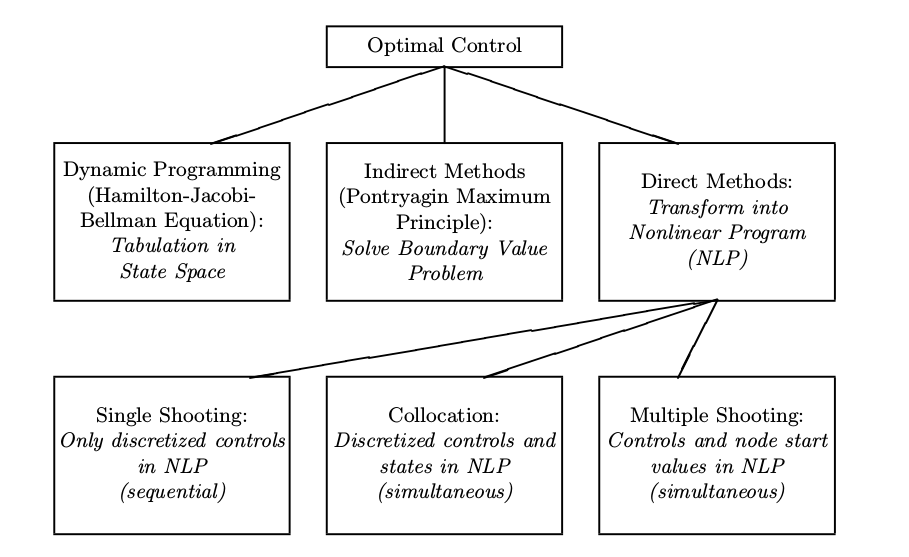
\includegraphics[width=120mm]{OptimizationDiehl}
  \caption{Different types of optimal control}
  \label{OptimizationDiehl}
\end{figure}
\end{itemize}
\textbf{Nonlinear Model Predictive Control} (NMPC) can be defined as a feedback technique aimed at solving a system . The dynamics of the system must be thus expressed as an optimization problem. The optimal solution is repeatedly computed at every time step of length $\delta = n \epsilon$ where $\epsilon$ is the calculation time (CPU time) of a single SQL iteration and $n$ is the number of need iterations to reach the convergence criterion.\\
\textbf{Online Dilemma}: A single SQP iteration (supposed it takes a constant time) can be solved in a time $\epsilon$ and we need $n$ iterations before the optimal convergence criterion can be met. This means that the solution for the initial condition $\hat{x}(t_k)$ can be found only at the instant $t_k + n \epsilon $. The system state at that instant will be probably different from $\hat{x}(t_k)$ (in the best case the state won't have changed much) so it could be useful to try to predict the most likely state at that instant. Also disturbance rejection, for the same reason, is applied with a delay $\delta_d = \delta$\\
\textbf{Real-time iteration scheme}